\documentclass[11pt]{article}
\usepackage[a4paper,margin=24mm]{geometry}
\usepackage[T1]{fontenc}
\usepackage[utf8]{inputenc}
\usepackage{lmodern,microtype}
\usepackage{amsmath,amssymb,amsthm,mathtools}
\usepackage{booktabs,tabularx,array,enumitem,placeins}
\usepackage{xcolor,hyperref,listings,tikz}
\usetikzlibrary{arrows.meta,positioning,fit}

\definecolor{navy}{HTML}{17365D}
\definecolor{teal}{HTML}{1F6F78}
\definecolor{soft}{HTML}{F2F5F7}
\definecolor{openred}{HTML}{9B3A32}
\hypersetup{colorlinks=true,linkcolor=navy,citecolor=teal,urlcolor=teal,
  pdftitle={Machine-Checked Haar and Differential Descent at an SU(2) Crossing: A Compensated-Flow Ward Identity},
  pdfauthor={Lluis Eriksson}}
\lstset{language={},basicstyle=\ttfamily\footnotesize,
  backgroundcolor=\color{soft},frame=single,rulecolor=\color{black!18},
  breaklines=true,columns=fullflexible,keepspaces=true,showstringspaces=false,
  xleftmargin=0.5em,xrightmargin=0.5em}

\newtheorem{theorem}{Theorem}[section]
\newtheorem{proposition}[theorem]{Proposition}
\newtheorem{corollary}[theorem]{Corollary}
\newtheorem{lemma}[theorem]{Lemma}
\theoremstyle{definition}
\newtheorem{definition}[theorem]{Definition}
\newtheorem{remark}[theorem]{Remark}

\newcommand{\SU}{\mathrm{SU}(2)}
\newcommand{\C}{\mathbb C}
\newcommand{\Haar}{\mu_{\mathrm H}}
\newcommand{\trn}{\operatorname{tr}_2}
\newcommand{\red}{\mathsf r}
\newcommand{\W}{\mathcal W}
\newcommand{\D}{\mathcal D}
\newcommand{\dir}{\mathrm{dir}}
\newcommand{\rev}{\mathrm{rev}}

\title{\vspace{-1.5em}\textbf{Machine-Checked Haar and Differential Descent at
an $\SU$ Crossing: A Four-Edge Compensated-Flow Ward Identity}}
\author{Lluis Eriksson}
\date{2 August 2026}

\begin{document}
\maketitle

\begin{abstract}
The local Makeenko--Migdal mechanism is usually expressed in two languages:
four holonomies on the edges incident to a crossing, and two effective group
coordinates on which invariant derivatives act.  We machine-check the exact
measure and differential bridge between them for $\SU$.  For
$a=(a_1,a_2,a_3,a_4)\in\SU^4$ we prove that
\[
 \red(a)=(a_2a_4^{-1},a_1a_3^{-1})
\]
pushes normalized four-fold Haar measure to normalized two-fold Haar measure,
and derive the corresponding integral identity for every strongly measurable
complex observable.  We then construct two gauge-compensated flows on the
literal four-edge chart.  They intertwine exactly with independent right
multiplication of the two quotient coordinates.  Consequently, first and
mixed derivatives of the crossing Wilson word descend without a gauge choice.
The three Pauli directions are proved individually, their
mixed generators close pointwise into direct and reverse trace resolutions,
and the previously established two-coordinate Ward identity is lifted to a
four-edge compensated-flow integral theorem with coefficients $-1/4$ and
$-1/2$.  This operator is not identified with the ordinary-edge mixed
operator of Driver--Hall--Kemp; the two have different reverse resolutions in
general.  The new Lean
producer contains 26 public declarations in 426 physical lines;
all 16 theorems have only the standard dependencies \texttt{propext},
\texttt{Classical.choice}, and \texttt{Quot.sound}.  No weak four-face
heat-kernel identity, alternating area derivative, or full
Makeenko--Migdal equation is claimed.
\end{abstract}

\section{Result and claim boundary}

For planar Yang--Mills theory, the Makeenko--Migdal relation converts an
alternating variation of the four face areas around a crossing into a local
second-order differential operator on edge holonomies.  The finite-dimensional
form of this mechanism is rigorous for suitable observables with extended
gauge invariance; see Driver--Hall--Kemp \cite{DHK} and the compact-surface
extension \cite{DGHK}.  Formalization forces a useful separation of four
interfaces:
\begin{enumerate}[leftmargin=1.7em,itemsep=0.2em]
 \item the physical four-edge chart and its normalized Haar measure;
 \item the two-coordinate differential Ward calculus;
 \item comparison with the ordinary-edge mixed operator used by
 Driver--Hall--Kemp;
 \item the analytic identification with four heat-kernel area derivatives.
\end{enumerate}
The present paper closes the first-to-second interface for the compensated
lift.  The third and fourth remain outside the theorem surface.
Table~\ref{tab:scope} is the claim ledger.

\begin{table}[ht]
\centering\small
\caption{Claim ledger. ``Checked'' means compiled in the new producer; an
imported row is a previously compiled theorem used by the endpoint.}
\label{tab:scope}
\begin{tabularx}{\textwidth}{@{}>{\raggedright\arraybackslash}X c
 >{\raggedright\arraybackslash}p{0.31\textwidth}@{}}
\toprule
Statement & Status & Mathematical role \\
\midrule
Four-edge quotient pushes $\Haar^{\otimes4}$ to $\Haar^{\otimes2}$
 & Checked & Exact measure descent \\
Integral quotient formula for measurable complex observables
 & Checked & Transfers expectations \\
Two gauge-compensated four-edge flows and intertwining laws
 & Checked & Exact differential interface \\
Generic first and mixed derivative descent
 & Checked & Coordinate-free generator transport \\
Six concrete Pauli derivative theorems
 & Checked & Reusable public calculus \\
Pauli trace--skein closure on the four-edge chart
 & Checked & Direct/reverse resolutions \\
Two-coordinate dominated-flow Ward identity
 & Imported & Finite-dimensional analytic input \\
Four-edge quotient-lifted compensated-flow Ward endpoint
 & Checked & Main theorem \\
Comparison with the ordinary-edge DHK mixed operator
 & Open & Distinct differential interface \\
Weak four-face heat-density identity and area differentiation
 & Open & Must incorporate the comparison \\
Full Makeenko--Migdal equation on an arbitrary cellulation
 & Open & Requires both open interfaces \\
\bottomrule
\end{tabularx}
\end{table}

This is a new sequel, not a replacement.  Its novelty is not another trace
calculation: it proves that the probability measure, the gauge-compensated
flows, and the differentiated Wilson observable commute with the same
quotient map and therefore support a single four-edge integral endpoint.

\section{The physical Haar quotient}

Let $a=(a_1,a_2,a_3,a_4)\in\SU^4$ list the four distinct outgoing edge
variables in cyclic order.  The local geometric word is
\begin{equation}\label{eq:word4}
 \W_4^{\alpha,\beta}(a)
   =\trn(a_3^{-1}\beta a_2a_4^{-1}\alpha a_1),
 \qquad \alpha,\beta\in\SU,
\end{equation}
where $\trn=\frac12\operatorname{Tr}$ is the normalized fundamental trace.
The quotient coordinates are
\begin{equation}\label{eq:red}
 \red(a)=(v_0,v_1)=(a_2a_4^{-1},a_1a_3^{-1}).
\end{equation}
They are the two physical entries of the full gauge-fixing chart
\begin{equation}\label{eq:fullchart}
 \Psi(a)=((a_2a_4^{-1},a_4),(a_1a_3^{-1},a_3)).
\end{equation}
The prior chart theorem proves that $\Psi$ preserves literal four-fold Haar.
Projection onto the first coordinate of each pair preserves the associated
product measure.  Composing these two measure-preserving maps yields the main
measure statement directly.

\begin{theorem}[Haar quotient]\label{thm:haar}
The map $\red:\SU^4\to\SU^2$ is measure preserving from
$\Haar^{\otimes4}$ to $\Haar^{\otimes2}$; equivalently,
\[
 \red_*\Haar^{\otimes4}=\Haar^{\otimes2}.
\]
\end{theorem}

The statement includes normalized measures on both sides; no hidden gauge
volume or proportionality constant is introduced.  It immediately produces
an integration theorem in the exact generality supported by the Bochner
integral.

\begin{corollary}[Exact quotient integration]\label{cor:integral}
If $F:\SU^2\to\C$ is almost-everywhere strongly measurable with respect to
$\Haar^{\otimes2}$, then
\begin{equation}\label{eq:integralquot}
 \int_{\SU^4}F(\red(a))\,d\Haar^{\otimes4}(a)
 =\int_{\SU^2}F(v)\,d\Haar^{\otimes2}(v).
\end{equation}
\end{corollary}

The result is stronger than checking the formula only for the Wilson word.
It is a reusable transport theorem for any physical density, derivative, or
resolved observable meeting the measurability hypothesis.

\section{Gauge-compensated physical flows}

Right multiplication of $v_0=a_2a_4^{-1}$ by a curve $\gamma(t)$ cannot be
realized by the naive change $a_2\mapsto a_2\gamma(t)$: the factor must pass
the return edge $a_4^{-1}$.  The correct physical insertion is its conjugate
by $a_4$.  Similarly, the second coordinate uses $a_3$.  Define
\begin{align}
 T_{0,t}^{\gamma}(a)
   &=\bigl(a_1,\ a_2(a_4^{-1}\gamma(t)a_4),\ a_3,\ a_4\bigr),
   \label{eq:flow0}\\
 T_{1,t}^{\gamma}(a)
   &=\bigl(a_1(a_3^{-1}\gamma(t)a_3),\ a_2,\ a_3,\ a_4\bigr).
   \label{eq:flow1}
\end{align}
For $R_{i,t}^{\gamma}$ denoting right multiplication of quotient coordinate
$i$ by $\gamma(t)$, cancellation gives the following exact identities.

\begin{theorem}[Intertwining]\label{thm:intertwine}
For every curve $\gamma:\mathbb R\to\SU$, time $t$, and configuration $a$,
\begin{equation}\label{eq:intertwine}
 \red(T_{0,t}^{\gamma}a)=R_{0,t}^{\gamma}(\red a),\qquad
 \red(T_{1,t}^{\gamma}a)=R_{1,t}^{\gamma}(\red a).
\end{equation}
\end{theorem}

\begin{figure}[ht]
\centering
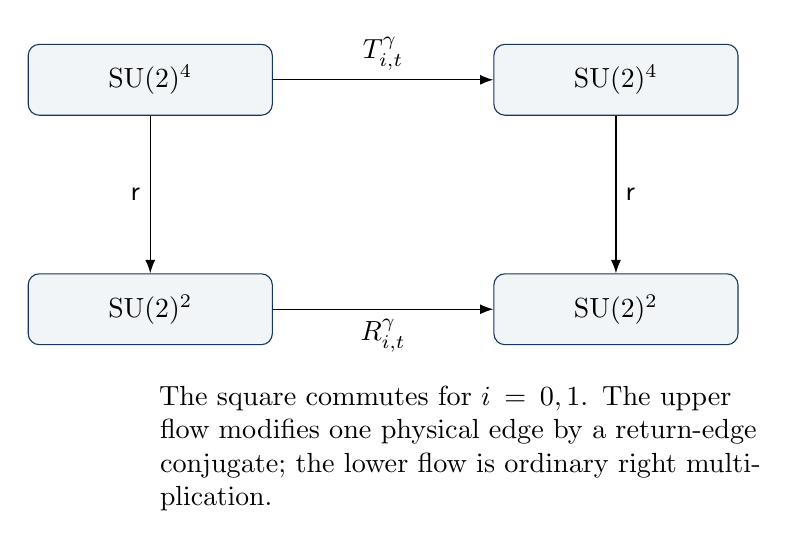
\begin{tikzpicture}[>=Latex,node distance=20mm and 28mm,
 box/.style={draw=navy,rounded corners,fill=soft,minimum width=31mm,
 minimum height=9mm,align=center},every edge/.style={draw,->}]
\node[box] (a0) {$\SU^4$};
\node[box,right=of a0] (b0) {$\SU^4$};
\node[box,below=of a0] (a1) {$\SU^2$};
\node[box,right=of a1] (b1) {$\SU^2$};
\path (a0) edge node[above] {$T_{i,t}^{\gamma}$} (b0)
      (a0) edge node[left] {$\red$} (a1)
      (b0) edge node[right] {$\red$} (b1)
      (a1) edge node[below] {$R_{i,t}^{\gamma}$} (b1);
\node[below=4mm of a1,anchor=north west,align=left,text width=78mm]
 {The square commutes for $i=0,1$.  The upper flow modifies one physical
 edge by a return-edge conjugate; the lower flow is ordinary right
 multiplication.};
\end{tikzpicture}
\caption{Exact flow descent.  Differentiation may be performed before or
after applying the quotient map.}
\label{fig:square}
\end{figure}

The conjugating factors are forced by \eqref{eq:red}; they are not a gauge
choice.  This distinction matters because the final integral remains over
all four edge variables with their literal product Haar law.

\section{Differential descent of the crossing word}

Set
\[
 \W_2^{\beta,\alpha}(v_0,v_1)=\trn(\beta v_0\alpha v_1).
\]
Cyclicity of the trace and \eqref{eq:red} give the already checked identity
\begin{equation}\label{eq:worddescent}
 \W_4^{\alpha,\beta}(a)=\W_2^{\beta,\alpha}(\red a).
\end{equation}
For a matrix tangent $X$, let $\D_0^X\W_2$ be the first right-invariant
generator, and for $X,Y$ let $\D_1^Y\D_0^X\W_2$ be the ordered mixed
generator.  The four-edge generators are defined by pullback:
\begin{align}
 \D_{4,0}^{X}\W_4(a)&=(\D_0^X\W_2)(\red a),\label{eq:first}\\
 \D_{4,1}^{Y}\D_{4,0}^{X}\W_4(a)
   &=(\D_1^Y\D_0^X\W_2)(\red a).\label{eq:mixed}
\end{align}

\begin{theorem}[Generic derivative descent]\label{thm:derivative}
Suppose $\gamma$ has entrywise derivative $X$ at zero.  Then
\[
 \left.\frac d{dt}\right|_{0}\W_4(T_{0,t}^{\gamma}a)
 =\D_{4,0}^{X}\W_4(a).
\]
If the entrywise derivative is $Y$, then
\[
 \left.\frac d{dt}\right|_{0}
   (\D_{4,0}^{X}\W_4)(T_{1,t}^{\gamma}a)
 =\D_{4,1}^{Y}\D_{4,0}^{X}\W_4(a).
\]
Both statements are formalized as \texttt{HasDerivAt} theorems.
\end{theorem}

The proof is a composition of \eqref{eq:intertwine},
\eqref{eq:worddescent}, and the earlier two-coordinate derivative theorem.
The producer then specializes both stages to the three anti-Hermitian Pauli
directions $X,Y,Z$, yielding six concrete public derivative theorems.  Thus
the generator language used in the Ward identity has a verified realization
as differentiation of the original four-edge holonomy.

\section{Compensated and ordinary-edge operators}

The preceding descent must not be confused with the ordinary-edge mixed
operator in Driver--Hall--Kemp.  Their operator differentiates the original
variables by
\[
 a_1\longmapsto a_1e^{sA},\qquad
 a_2\longmapsto a_2e^{tA},
\]
using the same Lie-algebra basis element $A$ at both edges.  On
\eqref{eq:word4}, the corresponding Pauli contraction is
\begin{equation}\label{eq:dhkop}
 C_{\mathrm{DHK}}(a)=\sum_{A\in\{X,Y,Z\}}
 \trn\!\left(a_3^{-1}\beta a_2 A
              a_4^{-1}\alpha a_1 A\right).
\end{equation}
By contrast, the quotient-lifted operator compiled here is
\begin{equation}\label{eq:qop}
 C_{\mathrm q}(a)=\sum_{A\in\{X,Y,Z\}}
 \trn\!\left(\beta a_2a_4^{-1}A
              \alpha a_1a_3^{-1}A\right).
\end{equation}
Equations~\eqref{eq:flow0}--\eqref{eq:flow1} show why: in the original edge
coordinates the two insertions are conjugated independently by $a_4^{-1}$
and $a_3^{-1}$.  Invariance of a Pauli contraction permits one common
orthogonal change of basis, not two unrelated adjoint rotations.  Hence
$C_{\mathrm q}$ and $C_{\mathrm{DHK}}$ are not equal in general.

The mismatch is also visible after trace--skein closure.  Both direct
resolutions equal the original crossing word, but the reverse resolutions
are different:
\begin{align}
 \W_{\mathrm{q,rev}}(a)
 &=\trn\!\left(\beta a_2a_4^{-1}a_3a_1^{-1}\alpha^{-1}\right),
 \label{eq:qrev}\\
 \W_{\mathrm{DHK,rev}}(a)
 &=\trn\!\left(a_3^{-1}\beta a_2a_1^{-1}\alpha^{-1}a_4\right).
 \label{eq:dhkrev}
\end{align}
The first is the pullback of the reverse resolution on the quotient.  The
second is formed from the two cut-loop holonomies
$a_3^{-1}\beta a_2$ and $a_4^{-1}\alpha a_1$.  The Lean theorem below concerns
\eqref{eq:qop} and \eqref{eq:qrev} only.  Establishing a relation to
\eqref{eq:dhkop}, most plausibly together with the concrete four-face thermal
density and its gauge-coordinate integration, is an explicit open interface.

\section{Trace--skein closure and the quotient-lifted Ward theorem}

Let $\W_{4,\dir}$ and $\W_{4,\rev}$ be the direct and reverse resolutions,
obtained by pulling the corresponding two-coordinate normalized-trace
pairings back along $\red$.  The fundamental $\SU$ completeness relation
gives a pointwise closure.

\begin{theorem}[Pauli closure]\label{thm:closure}
For every $a\in\SU^4$,
\begin{equation}\label{eq:closure}
 \sum_{A\in\{X,Y,Z\}}\D_{4,1}^{A}\D_{4,0}^{A}\W_4(a)
 =-\frac14\W_{4,\dir}(a)-\frac12\W_{4,\rev}(a).
\end{equation}
\end{theorem}

The coefficients reflect the chosen Pauli normalization and normalized
fundamental trace.  They are compiled constants, not inferred from numerical
experiments.

For the integral theorem, write $\rho:\SU^2\to\C$ for a physical density and
$D_1D_2\rho_A$ for its mixed derivative in Pauli direction $A$.  The Lean
structure \texttt{SU2CrossingPauliWardData} packages $\rho$, the six derivative
functions, and exactly six \texttt{DominatedFlowPair} certificates.  These
certificates provide the measurability, integrability, product rule, and
dominated differentiation required by two integrations by parts.  They are
assumptions of the endpoint, not assertions about a heat-kernel density.

\begin{theorem}[Four-edge quotient-lifted compensated-flow Ward identity]
\label{thm:ward}
For $\alpha,\beta\in\SU$ and any certified Ward data $D$,
\begin{align}
 &\int_{\SU^4}\left(\sum_{A=X,Y,Z}D_1D_2\rho_A(\red a)\right)
       \W_4^{\alpha,\beta}(a)\,d\Haar^{\otimes4}(a) \notag\\
 &\quad=\int_{\SU^4}\rho(\red a)
   \left[-\frac14\W_{4,\dir}^{\alpha,\beta}(a)
         -\frac12\W_{4,\rev}^{\alpha,\beta}(a)\right]
       d\Haar^{\otimes4}(a).\label{eq:ward4}
\end{align}
\end{theorem}

The proof transports the left integrand to $\SU^2$ using
Corollary~\ref{cor:integral}, applies the machine-checked two-coordinate Ward
identity, uses Theorem~\ref{thm:closure}, and transports the result back.  The
two uses of quotient integration require separate measurability proofs; both
are discharged from the fields of the dominated-flow certificates.

Equation~\eqref{eq:ward4} is the strongest unconditional conclusion of this
paper.  Calling its mixed operator the ordinary-edge operator
\eqref{eq:dhkop}, or calling its left side an alternating four-area
derivative, would require further comparison and heat-kernel theorems.  No
such identification appears in the Lean statement or manuscript.

\section{Proof design and reusable consequences}

The endpoint is assembled from four independently reusable transports.  This
factorization identifies exactly where a future heat-kernel theorem must
enter.

\paragraph{Measure transport.}
The proof of Theorem~\ref{thm:haar} does not expand a Haar integral by hand.
It composes the verified full chart $\Psi$ with the two projections
$(v,g)\mapsto v$.  Projection from a product probability measure is measure
preserving, and the equivalence between pairs and functions on
\texttt{Fin 2} supplies the last representation change.  The argument is
therefore stable under replacement of the integrand and independent of trace
identities.

\paragraph{Observable transport.}
Equation~\eqref{eq:worddescent} was established before the new module, but the
current proof uses it at the integral endpoint rather than only as a
pointwise simplification.  The left integrand in \eqref{eq:ward4} is first
identified almost everywhere with a composite $F_L\circ\red$ and transferred
by Corollary~\ref{cor:integral}.  After the two-coordinate Ward theorem, a
separately constructed $F_R\circ\red$ is transferred back.  Keeping $F_L$
and $F_R$ distinct prevents a hidden assumption that the closed resolution
is measurable merely because the unclosed derivative sum is measurable; the
proof establishes this through the pointwise Pauli identity.

\paragraph{Differential transport.}
The flows \eqref{eq:flow0} and \eqref{eq:flow1} literally realize quotient
differentiation on the original edges.  For example,
\[
 a_2(a_4^{-1}\gamma a_4)a_4^{-1}
   =(a_2a_4^{-1})\gamma.
\]
The return-edge conjugation is forced by the quotient formula.  Once
Theorem~\ref{thm:intertwine} is available, the generic
\texttt{HasDerivAt} endpoints follow by rewriting the complete curve rather
than redoing matrix differentiation in four variables.  The six Pauli
theorems instantiate this common interface without extra assumptions.

\paragraph{Hypothesis transport.}
The structure $D$ deliberately lives on $\SU^2$.  Its six dominated-flow
certificates are exactly those consumed by the earlier integration-by-parts
theorem: two coordinate directions for each of three Pauli axes.  The new
four-edge theorem neither duplicates these certificates nor postulates that
a four-variable density has unexplained derivatives.  It integrates the
pullback $\rho\circ\red$ against $\Haar^{\otimes4}$.  Any future construction
of heat-kernel Ward data on the quotient can therefore be inserted unchanged
into Theorem~\ref{thm:ward}.

Two reusable consequences are immediate.  Any physical observable factoring
through $\red$ inherits the exact Haar quotient formula.  Also, any matrix
tangent curve with an entrywise derivative may use the generic differential
endpoints; the Pauli basis is required only for the completeness relation
\eqref{eq:closure}.  These are public interfaces for subsequent
formalization, not auxiliary steps hidden inside the headline proof.

\section{Formal architecture and audit}

The new producer imports the prior extended-gauge chart, which itself imports
the concrete $\SU$ Haar, derivative, trace--skein, and Ward layers.  The
resulting proof path is shown in Figure~\ref{fig:pipeline}.  The dashed boxes
separate the ordinary-edge operator comparison from the heat-density step;
neither is silently absorbed into the compiled path.

\begin{figure}[ht]
\centering
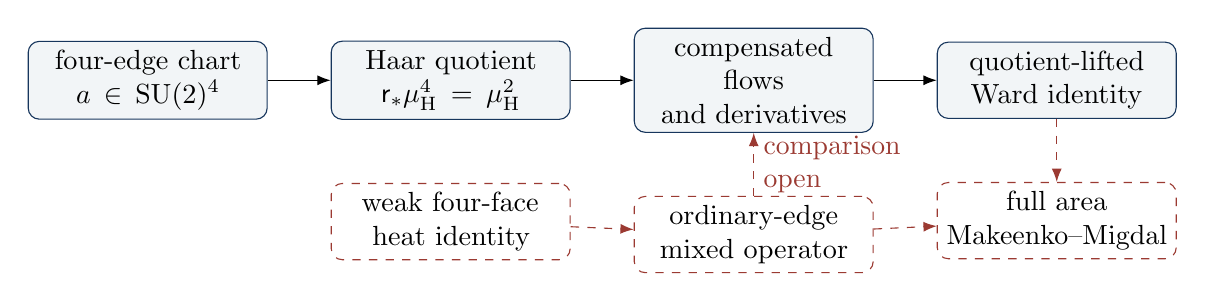
\begin{tikzpicture}[>=Latex,node distance=8mm and 8mm,
 n/.style={draw=navy,rounded corners,fill=soft,align=center,
 minimum height=8mm,text width=28mm},
 o/.style={draw=openred,dashed,rounded corners,align=center,
 minimum height=8mm,text width=28mm}]
\node[n] (chart) {four-edge chart\\$a\in\SU^4$};
\node[n,right=of chart] (haar) {Haar quotient\\$\red_*\Haar^4=\Haar^2$};
\node[n,right=of haar] (flow) {compensated flows\\and derivatives};
\node[n,right=of flow] (ward) {quotient-lifted\\Ward identity};
\node[o,below=of haar] (area) {weak four-face\\heat identity};
\node[o,below=of flow] (ordinary) {ordinary-edge\\mixed operator};
\node[o,below=of ward] (mm) {full area\\Makeenko--Migdal};
\draw[->] (chart)--(haar);
\draw[->] (haar)--(flow);
\draw[->] (flow)--(ward);
\draw[->,dashed,openred] (area)--(ordinary);
\draw[->,dashed,openred] (ordinary)--(mm);
\draw[->,dashed,openred] (ordinary)--node[right,align=left]
  {comparison\\open} (flow);
\draw[->,dashed,openred] (ward)--(mm);
\end{tikzpicture}
\caption{Compiled compensated-flow path (solid).  The ordinary-edge
comparison and heat-density extension remain open (dashed).}
\label{fig:pipeline}
\end{figure}

Table~\ref{tab:lean} maps the paper statements to the public Lean surface.
The producer has 426 physical lines and 26 public declarations: nine
definitions, one structure, and 16 theorems.

\begin{table}[ht]
\centering\scriptsize
\caption{Paper-to-Lean map for the new producer.}
\label{tab:lean}
\begin{tabularx}{\textwidth}{@{}p{0.29\textwidth}X p{0.17\textwidth}@{}}
\toprule
Paper result & Lean declaration & Kind \\
\midrule
Haar quotient, Thm.~\ref{thm:haar}
 & \texttt{su2CrossingReducedConfiguration\_measurePreserving} & theorem \\
Integral quotient, Cor.~\ref{cor:integral}
 & \texttt{integral\_su2CrossingReducedConfiguration} & theorem \\
Physical flows, \eqref{eq:flow0}--\eqref{eq:flow1}
 & \texttt{su2CrossingPhysicalFlow0}, \texttt{...Flow1} & definitions \\
Intertwining, Thm.~\ref{thm:intertwine}
 & \texttt{su2CrossingReducedConfiguration\_physicalFlow0/1} & 2 theorems \\
Generic differential descent, Thm.~\ref{thm:derivative}
 & \texttt{hasDerivAt\_su2FourEdgeCrossing...\_zero} & 2 theorems \\
Concrete Pauli calculus
 & \texttt{hasDerivAt\_su2FourEdgeCrossing...\_pauliX/Y/Z} & 6 theorems \\
Pauli closure, Thm.~\ref{thm:closure}
 & \texttt{su2FourEdgeCrossingMixedGenerator\_pauli\_sum\_closed} & theorem \\
Ward hypotheses
 & \texttt{SU2CrossingPauliWardData} & structure \\
Quotient-lifted endpoint, Thm.~\ref{thm:ward}
 & \texttt{integral\_su2FourEdgeCrossing\_pauliWard\_closed} & theorem \\
\bottomrule
\end{tabularx}
\end{table}

The dedicated audit invokes \texttt{\#print axioms} on every new theorem.
Each report contains exactly the standard logical dependencies
\texttt{propext}, \texttt{Classical.choice}, and \texttt{Quot.sound}.  A
clean-source wrapper pins Lean \texttt{v4.29.0-rc6} and Mathlib commit
\texttt{07642720480157414db592fa85b626d\allowbreak{}afb71355b}, builds the
full 2915-job
dependency closure, compiles the audit, rejects \texttt{sorry},
\texttt{admit}, and local \texttt{axiom} in the two new modules, checks the
line and declaration counts, and records SHA-256 hashes.

\FloatBarrier
\section{Conclusion}

The four-edge crossing chart and the two-coordinate Ward chart are now linked
by more than an algebraic equality of Wilson words.  Their probability laws
agree under an exact Haar pushforward; quotient right-invariant directions
have explicit gauge-compensated lifts; and the Pauli-summed Ward identity
returns to a literal four-edge integral with its quotient direct/reverse
coefficients intact.  This closes the compensated quotient-lift and no more.
The comparison with the ordinary-edge Driver--Hall--Kemp operator, the
heat-kernel four-area identity, arbitrary-cellulation geometry, and the full
Makeenko--Migdal equation remain future work.

\begin{thebibliography}{9}
\bibitem{MM}
Y.~Makeenko and A.~Migdal,
Exact equation for the loop average in multicolor QCD,
\emph{Physics Letters B} \textbf{88} (1979), 135--137.

\bibitem{DHK}
B.~K. Driver, B.~C. Hall, and T.~Kemp,
Three proofs of the Makeenko--Migdal equation for Yang--Mills theory on the
plane,
\emph{Communications in Mathematical Physics} \textbf{351} (2017), 741--774;
\href{https://arxiv.org/abs/1601.06283}{arXiv:1601.06283}.

\bibitem{DGHK}
B.~K. Driver, F.~Gabriel, B.~C. Hall, and T.~Kemp,
The Makeenko--Migdal equation for Yang--Mills theory on compact surfaces,
\emph{Communications in Mathematical Physics} \textbf{352} (2017), 967--978;
\href{https://arxiv.org/abs/1602.03905}{arXiv:1602.03905}.

\bibitem{Levy}
T.~L\'evy,
The master field on the plane,
\emph{Ast\'erisque} \textbf{388} (2017).

\bibitem{Lean}
L.~de Moura and S.~Ullrich,
The Lean 4 theorem prover and programming language,
in \emph{Automated Deduction -- CADE 28}, LNCS 12699, Springer, 2021,
625--635.

\bibitem{Mathlib}
The Mathlib Community,
The Lean mathematical library,
in \emph{Proceedings of CPP 2020}, ACM, 2020, 367--381.
\end{thebibliography}

\end{document}
